\clearpage
\subsubsection{UCA 5 - Monitoraggio dello storico degli accessi dell'utente}

\begin{figure}[h]
	\centering	
	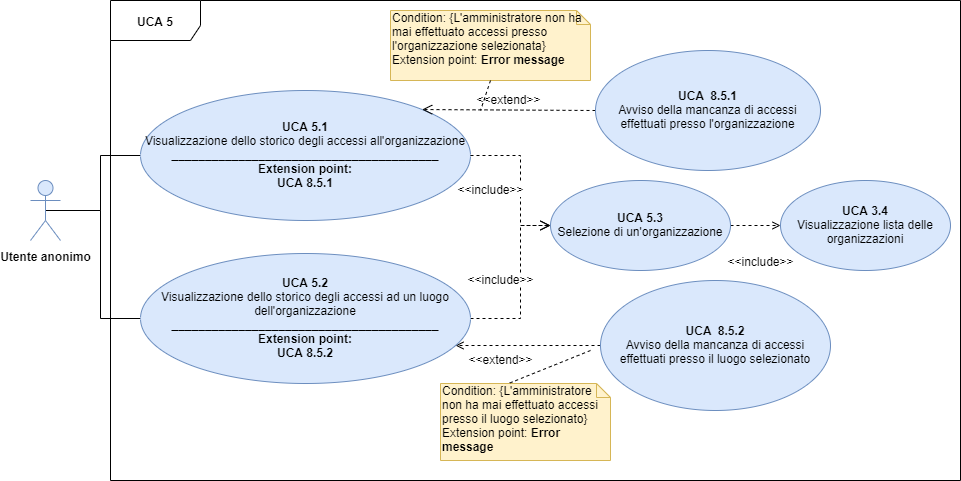
\includegraphics[scale=0.6]{Sezioni/UseCase/Immagini/UCA5.png}
	\caption{UCA 5 - Monitoraggio dello \glo{storico degli accessi} dell'utente}
\end{figure}

\begin{itemize}
    \item \textbf{Attori primari:} Utente anonimo
    \item \textbf{Precondizione:} L'utente ha precedentemente scaricato la lista delle \glo{organizzazioni}.
    \item \textbf{Postcondizione:} L'utente ha visualizzato lo \glo{storico degli accessi} relativo all'\glo{organizzazione} desiderata oppure al \glo{luogo} desiderato dell'\glo{organizzazione} scelta.
    \item \textbf{Scenario principale:} L'utente selezionerà l'\glo{organizzazione} desiderata dalla lista delle \glo{organizzazioni} e quindi la funzionalità per mostrare lo \glo{storico degli accessi} oppure un \glo{luogo} specifico per analizzarne il relativo \glo{storico degli accessi}. Inoltre ha la possibilità di ordinare gli accessi o effettuare ricerche.
\end{itemize}
\newpage
\subsubsection{UCA 5.1 - Visualizzazione dello storico degli accessi all'organizzazione}

\begin{figure}[h]
	\centering	
	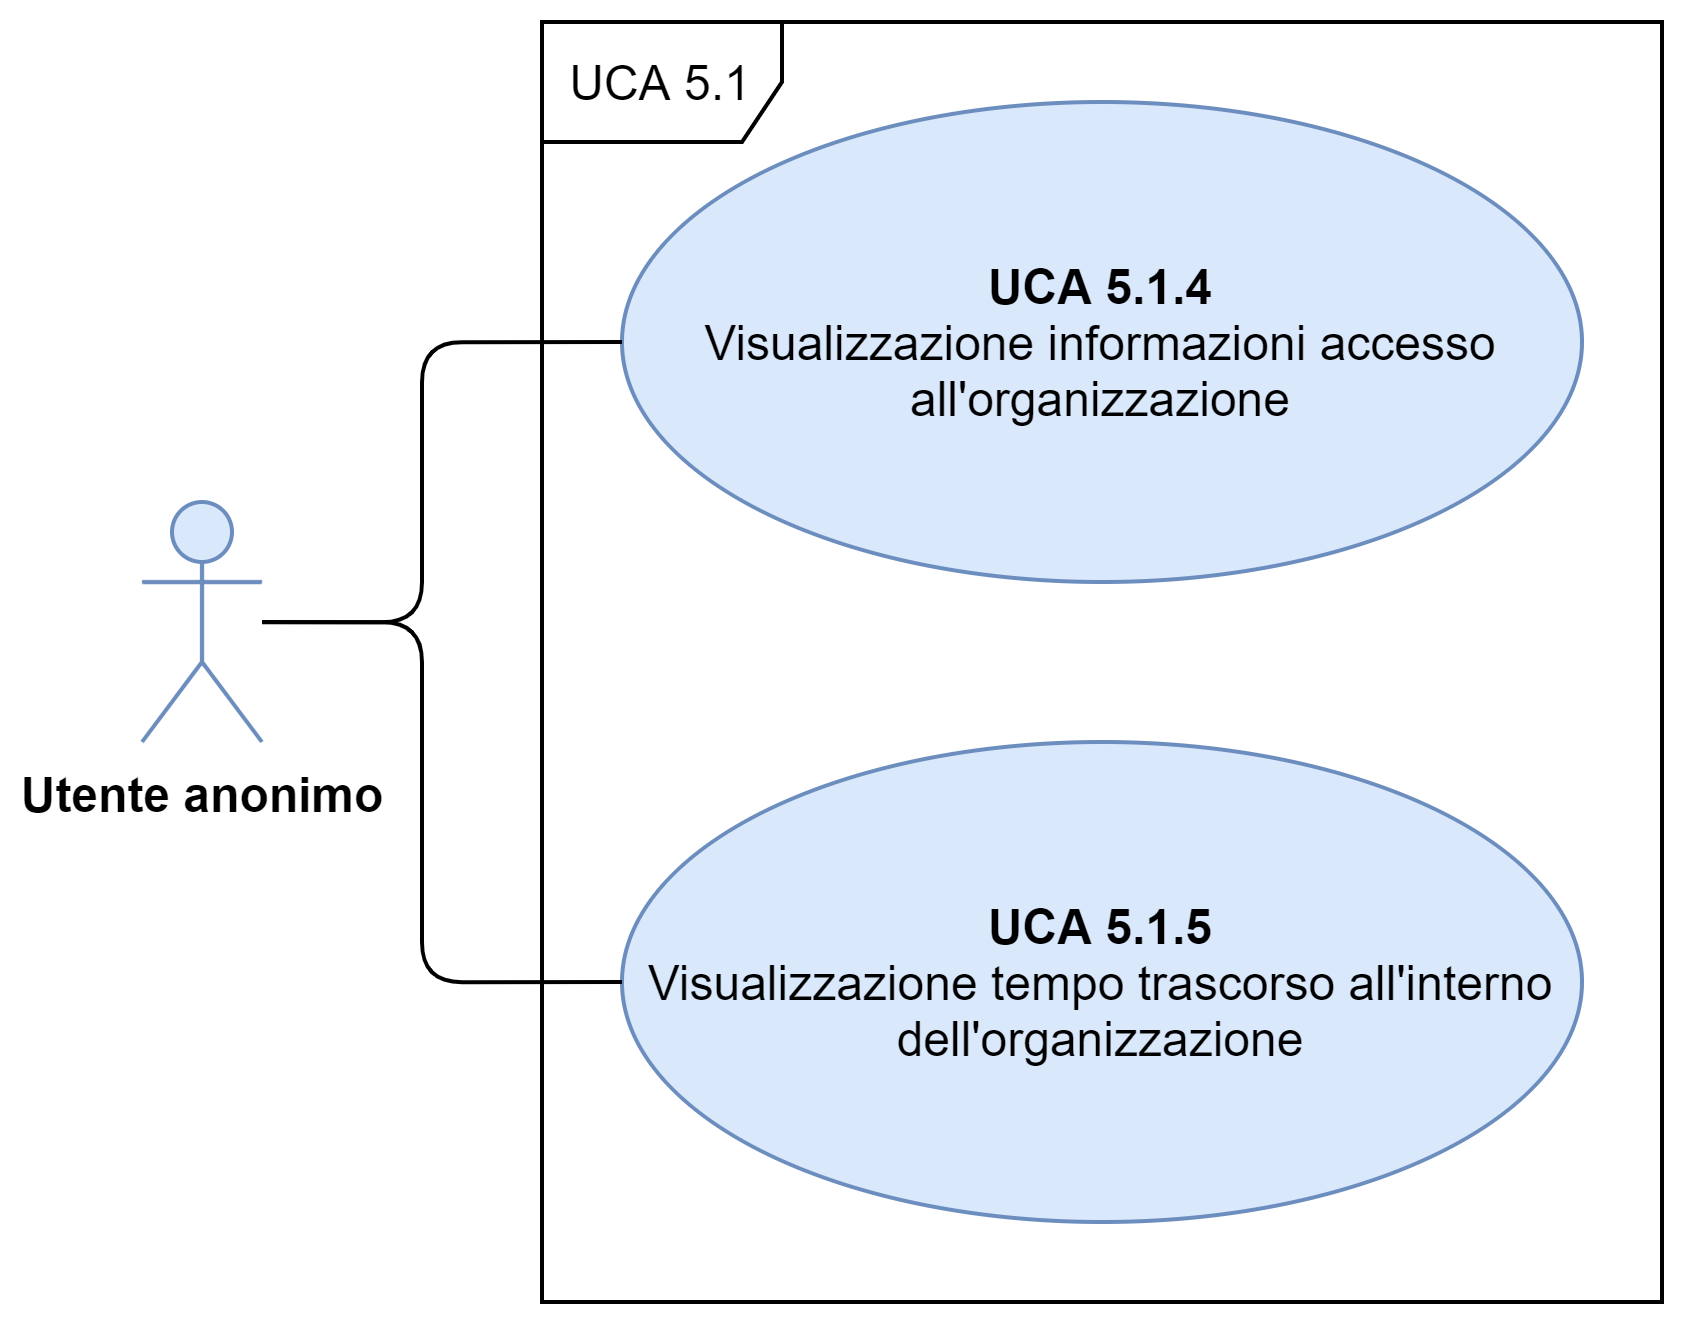
\includegraphics[scale=0.6]{Sezioni/UseCase/Immagini/UCA5.1.png}
	\caption{UCA 5.1 - Visualizzazione dello \glo{storico degli accessi} all'organizzazione}
\end{figure}

\begin{itemize}
    \item \textbf{Attori primari:} Utente anonimo
    \item \textbf{Precondizione:} L'utente dispone della lista delle \glo{organizzazioni}.
    \item \textbf{Postcondizione:} L'utente ha visualizzato lo \glo{storico degli accessi} presso l'\glo{organizzazione} scelta.
    \item \textbf{Scenario principale:} L'utente esegue la procedura per visualizzare lo \glo{storico degli accessi} effettuati presso l'\glo{organizzazione} selezionata.
    \item \textbf{Scenario alternativo:} L'utente non è mai entrato nell'\glo{organizzazione} selezionata, pertanto verrà visualizzato un avviso informativo [UCA 8.5.1].
    \item \textbf{Flusso di eventi:}
    \begin{enumerate}
        \item L'utente seleziona la funzionalità per mostrare gli accessi effettuati presso un'\glo{organizzazione} [UCA 5.1.4] oppure visualizza il tempo trascorso all'interno dell'organizzazione [UCA 5.1.5];
        \item L'utente visiona per ogni accesso le sue informazioni.
    \end{enumerate}
    \item \textbf{Estensioni:}
    \begin{itemize}
        \item UCA 8.5.1 - Avviso della mancanza di accessi effettuati presso l'organizzazione selezionata.
    \end{itemize}
\end{itemize}

\subsubsection{UCA 5.1.4 - Visualizzazione informazioni accesso all'organizzazione}
\begin{itemize}
	\item \textbf{Attori primari:} Utente anonimo
	\item \textbf{Precondizione:} L'utente sta visionando un accesso ad un'\glo{organizzazione}.
	\item \textbf{Postcondizione:} L'utente visiona le informazioni relative all'accesso effettuato.
	\item \textbf{Scenario principale:} Viene visualizzato il timestamp di ingresso, di uscita e il tempo di permanenza presso l'organizzazione.
\end{itemize}

\subsubsection{UCA 5.1.5 - Visualizzazione tempo trascorso all'interno dell'organizzazione}
\begin{itemize}
	\item \textbf{Attori primari:} Utente anonimo
	\item \textbf{Precondizione:} L'utente ha selezionato l'organizzazione e si trova fisicamente al suo interno.
	\item \textbf{Postcondizione:} Viene visualizzato il tempo trascorso all'interno dell'organizzazione dall'ultimo ingresso.
	\item \textbf{Scenario principale:} Viene visualizzato il tempo trascorso all'interno dell'organizzazione dall'ultimo ingresso.
\end{itemize}

\subsubsection{UCA 5.2 - Visualizzazione dello storico degli accessi ad un luogo dell'organizzazione}

\begin{figure}[h]
	\centering	
	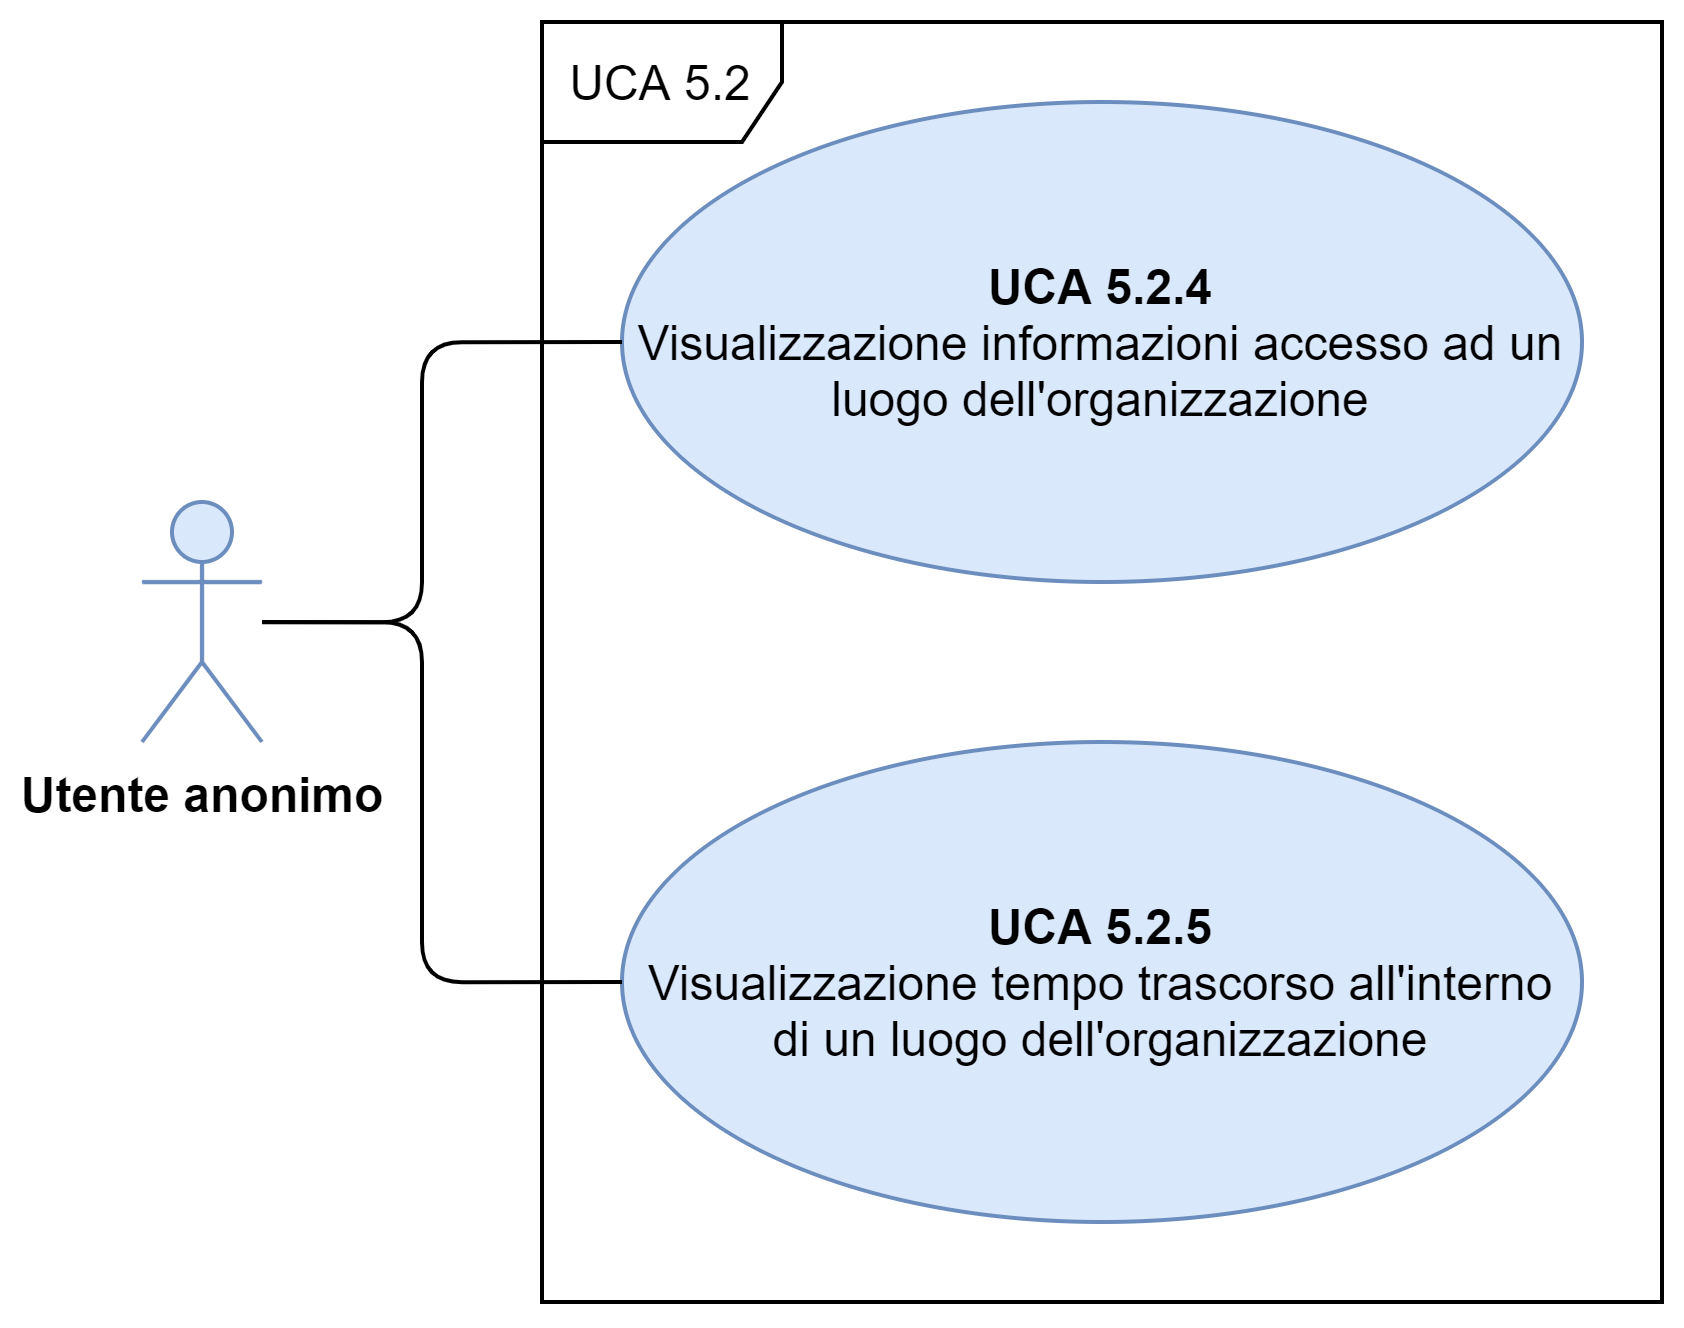
\includegraphics[scale=0.6]{Sezioni/UseCase/Immagini/UCA5.2.png}
	\caption{UCA 5.2 - Visualizzazione dello \glo{storico degli accessi} ad un luogo dell'organizzazione}
\end{figure}

\begin{itemize}
    \item \textbf{Attori primari:} Utente anonimo
    \item \textbf{Precondizione:} L'utente seleziona il luogo dell'\glo{organizzazione} di cui vuole visualizzare i propri accessi.
    \item \textbf{Postcondizione:} L'utente visualizza lo \glo{storico degli accessi} (con nome del \glo{luogo}, \glo{timestamp} di ingresso, di uscita e tempo di permanenza) al \glo{luogo} desiderato. Se l'utente dovesse trovarsi all'interno del \glo{luogo} stesso, viene visualizzato il tempo passato al suo interno dall'ultimo ingresso effettuato.
    \item \textbf{Scenario principale:} L'utente esegue la procedura per visualizzare lo \glo{storico degli accessi} effettuati presso il \glo{luogo} selezionato.
    \item \textbf{Scenario alternativo:} L'utente non è mai entrato nel \glo{luogo} selezionato, pertanto verrà mostrato un avviso informativo [UCA 8.5.2].
    \item \textbf{Flusso di eventi:}
    \begin{enumerate}
    	\item L'utente seleziona la funzionalità per mostrare gli accessi effettuati presso un \glo{luogo} di un'\glo{organizzazione} [UCA 5.2.4] oppure visualizza il tempo trascorso all'interno del luogo [UCA 5.2.5];
    	\item L'utente visiona per ogni accesso le sue informazioni.
    \end{enumerate}
    \item \textbf{Estensioni:}
    \begin{itemize}
        \item UCA 8.5.2 - Avviso della mancanza di accessi effettuati presso il luogo selezionato.
    \end{itemize}
\end{itemize}

\subsubsection{UCA 5.2.4 - Visualizzazione informazioni accesso ad un luogo dell'organizzazione}
\begin{itemize}
	\item \textbf{Attori primari:} Utente anonimo
	\item \textbf{Precondizione:} L'utente sta visionando un accesso ad un luogo dell'\glo{organizzazione}.
	\item \textbf{Postcondizione:} L'utente visiona le informazioni relative all'accesso effettuato.
	\item \textbf{Scenario principale:} Viene visualizzato il timestamp di ingresso, di uscita e il tempo di permanenza presso il luogo dell'organizzazione.
\end{itemize}

\subsubsection{UCA 5.2.5 - Visualizzazione tempo trascorso all'interno di un luogo dell'organizzazione}
\begin{itemize}
	\item \textbf{Attori primari:} Utente anonimo
	\item \textbf{Precondizione:} L'utente ha selezionato un luogo dell'organizzazione e si trova fisicamente al suo interno.
	\item \textbf{Postcondizione:} Viene visualizzato il tempo trascorso all'interno del luogo dell'organizzazione dall'ultimo ingresso.
	\item \textbf{Scenario principale:} Viene visualizzato il tempo trascorso all'interno del luogo dell'organizzazione dall'ultimo ingresso.
\end{itemize}

\subsubsection{UCA 5.4 - Ordinamento per data della lista degli accessi presso un'organizzazione o un suo luogo}
\begin{itemize}
    \item \textbf{Attori primari:} Utente anonimo
    \item \textbf{Precondizione:} L'utente seleziona la visualizzazione della lista degli accessi ordinata per data.
    \item \textbf{Postcondizione:} L'utente ottiene la \glo{lista degli accessi} riordinata \glo{per data}.
    \item \textbf{Scenario principale:} Ordinamento per data della lista degli accessi in un determinato ordine.
\end{itemize}

\subsubsection{UCA 5.4.1 - Ordinamento per data decrescente della lista degli accessi presso un'organizzazione o un suo luogo}
\begin{itemize}
	\item \textbf{Attori primari:} Utente anonimo
	\item \textbf{Precondizione:} L'utente seleziona la visualizzazione della lista degli accessi ordinata per data decrescente.
	\item \textbf{Postcondizione:} L'utente ottiene la \glo{lista degli accessi} riordinata \glo{per data in ordine decrescente}.
	\item \textbf{Scenario principale:} Ordinamento per data decrescente della lista degli accessi.
	\item \textbf{Generalizzazione:}
	\begin{enumerate}
		\item UCA 5.4 - Ordinamento per data della lista degli accessi presso un'organizzazione o un suo luogo.
	\end{enumerate} 
\end{itemize}

\subsubsection{UCA 5.4.2 - Ordinamento per data crescente della lista degli accessi presso un'organizzazione o un suo luogo}
\begin{itemize}
    \item \textbf{Attori primari:} Utente anonimo
    \item \textbf{Precondizione:} L'utente seleziona la visualizzazione della lista degli accessi ordinata per data crescente.
    \item \textbf{Postcondizione:} L'utente ottiene la \glo{lista degli accessi} riordinata \glo{per data crescente}.
    \item \textbf{Scenario principale:} Ordinamento per data crescente della lista degli accessi.
    \item \textbf{Generalizzazione:}
	\begin{enumerate}
		\item UCA 5.4 - Ordinamento per data della lista degli accessi presso un'organizzazione o un suo luogo.
	\end{enumerate}
\end{itemize}

\subsubsection{UCA 5.5 - Ricerca degli accessi presso un'organizzazione o un suo luogo in un giorno specifico}
\begin{itemize}
    \item \textbf{Attori primari:} Utente anonimo
    \item \textbf{Precondizione:} L'utente sta visionando lo storico accessi di un \glo{luogo}.
    \item \textbf{Postcondizione:} L'utente ottiene la \glo{lista degli accessi} effettuati presso il \glo{luogo} in questione nel giorno selezionato.
    \item \textbf{Scenario principale:} Ricerca degli accessi presso un'organizzazione o un suo luogo in un giorno specifico.
\end{itemize}